% ADMD 2026 one-page abstract. Compile with XeLaTeX.
\documentclass[11pt,a4paper]{article}
\usepackage[margin=20mm]{geometry}
\usepackage{fontspec}
% The final PDF embeds Times New Roman. Put Times.TTF, Timesbd.TTF,
% Timesi.TTF, and Timesbi.TTF in /tmp/times-fonts/ before compiling.
\setmainfont[
  Path=/tmp/times-fonts/,
  UprightFont=Times.TTF,
  BoldFont=Timesbd.TTF,
  ItalicFont=Timesi.TTF,
  BoldItalicFont=Timesbi.TTF
]{Times New Roman}
\usepackage{microtype}
\usepackage{amsmath}
\usepackage{xcolor}
\usepackage{tikz}
\usetikzlibrary{arrows.meta,positioning,calc,fit}
\usepackage{pgfplots}
\pgfplotsset{compat=1.18}
\usepackage[hidelinks]{hyperref}

\definecolor{navy}{HTML}{12304A}
\definecolor{teal}{HTML}{008C8C}
\definecolor{aqua}{HTML}{4FC3B3}
\definecolor{gold}{HTML}{E7A93B}
\definecolor{coral}{HTML}{D95F59}
\definecolor{paleblue}{HTML}{EAF1F8}
\definecolor{ink}{HTML}{17242F}

\color{ink}
\pagestyle{empty}
\setlength{\parindent}{0pt}
\setlength{\parskip}{2.5pt}
\setlength{\emergencystretch}{1em}
\newcommand{\tightheading}[1]{\vspace{1pt}{\bfseries\color{navy}#1}\par\vspace{-2pt}}

\begin{document}

\begin{center}
{\fontsize{15.5}{17}\selectfont\bfseries\color{navy}
Graph-Attention Surrogates for Variational Circuit Selection\\
Across Molecular Geometries and Correlation Regimes\par}
\vspace{3pt}
{\bfseries Syed Mohaiminul Hoque}\\
Center for Computational and Data Sciences, Independent University Bangladesh\\
\href{mailto:syedmuhaimintahsin@gmail.com}{syedmuhaimintahsin@gmail.com}
\end{center}
\vspace{-2pt}

\tightheading{Abstract}
Selecting expressive variational circuits without exhaustively optimizing every
candidate is a central bottleneck in VQE-based quantum chemistry and
correlated-electron simulation. We ask whether
graph-attention surrogates can rank particle-number-preserving ans\"atze when both the
circuit architecture and Hamiltonian parameter are unseen.

We benchmark four-qubit half-filled two-site Fermi--Hubbard Hamiltonians and six-qubit
active-space LiH in STO--3G. Full runs comprise 1,080 Hubbard and 810 LiH VQE labels
with paired optimizer initializations. A lossless Pauli-factor graph retains every
aggregated Pauli word, axis, and coefficient; circuit graphs encode excitation order
and wires. Edge-conditioned GAT models with MLP or KAN heads learn
within-Hamiltonian standardized energies under fingerprint-disjoint splits:
\vspace{-3pt}
\[
 a^*(H)=\arg\min_a\min_{\boldsymbol\theta}
 \langle\psi_a(\boldsymbol\theta)|H|\psi_a(\boldsymbol\theta)\rangle,
 \qquad \Delta E_a=E_a^{\mathrm{VQE}}-E_0.
\]
\vspace{-7pt}

For Hubbard, one simultaneous-transfer split reached Kendall
\(\tau_b=0.569\), but the five-seed mean was only \(0.180\)
(SD \(0.415\), bootstrap 95\% CI \([-0.120,0.540]\)), revealing substantial
seed sensitivity. On unseen LiH circuits and geometries, circuit GAT led
(\(\tau_b=0.259,\rho=0.366\)); factor-GAT+KAN was close
(\(\tau_b=0.233,\rho=0.362\)), while Hamiltonian encodings provided no clear
advantage. The median LiH gap exceeded 1.6 mHa from 2.4 \AA, whereas the best sampled
circuit stayed below this threshold throughout. High-precision finalist reruns changed
LiH gaps by at most \(3.13\times10^{-6}\) Ha. Together, these results show that
graph-attention surrogates can support variational-circuit selection across molecular
and correlated-electron Hamiltonians, while seed sensitivity makes leakage-controlled
validation essential. By screening ans\"atze before costly VQE optimization, the
framework could reduce the number of full optimizations required across molecular
geometry scans and correlated-electron parameter sweeps---repeated tasks in
quantum-chemical potential-energy surfaces and materials-relevant electronic-structure
workflows.

\vspace{1pt}
\begin{center}
\begin{tikzpicture}[
  font=\fontsize{7.5}{8.5}\selectfont,
  box/.style={rounded corners=1.2mm,draw=navy!70,fill=paleblue,
              minimum height=9mm,text width=29mm,align=center,inner sep=.8mm},
  arr/.style={-{Stealth[length=1.6mm]},draw=teal,line width=.85pt}
]
\node[box,fill=gold!16] (h) {\textbf{Hamiltonians}\\Hubbard (4q) + LiH (6q)};
\node[box,right=4mm of h] (d) {\textbf{1,890 VQE labels}\\paired initialization};
\node[box,right=4mm of d] (g) {\textbf{Joint graphs}\\circuit + Pauli factors};
\node[box,right=4mm of g] (m) {\textbf{GAT / KAN}\\same-\(H\) ranking loss};
\node[box,right=4mm of m,fill=aqua!16] (v) {\textbf{Held-out test}\\architecture + geometry};
\draw[arr] (h)--(d); \draw[arr] (d)--(g); \draw[arr] (g)--(m); \draw[arr] (m)--(v);

\node[anchor=north west] at ([yshift=-5mm]h.south west) {
\begin{tikzpicture}
\begin{axis}[
 width=76mm,height=43mm,ybar,bar width=9pt,
 ymin=0,ymax=.32,ylabel={Macro Kendall $\tau_b$},
 symbolic x coords={Circuit,Pairwise,Factor,F+KAN},xtick=data,
 ytick={0,.1,.2,.3},grid=major,grid style={gray!16},
 tick label style={font=\fontsize{7}{8}\selectfont},
 label style={font=\fontsize{7.5}{8.5}\selectfont},
 title={\textbf{Unseen LiH circuits + geometries}},
 title style={font=\fontsize{8.5}{9.5}\selectfont},
 nodes near coords,nodes near coords style={font=\fontsize{6.8}{7.6}\selectfont},
 enlarge x limits=.16]
\addplot[fill=teal!75,draw=teal] coordinates
 {(Circuit,.259259) (Pairwise,.202614) (Factor,.137255) (F+KAN,.233115)};
\end{axis}
\end{tikzpicture}};

\node[anchor=north east] at ([yshift=-5mm]v.south east) {
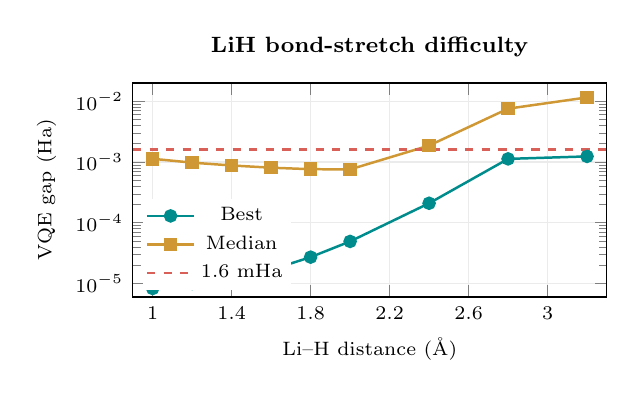
\begin{tikzpicture}
\begin{semilogyaxis}[
 width=76mm,height=43mm,
 xmin=.9,xmax=3.3,ymin=6e-6,ymax=2e-2,
 xlabel={Li--H distance (\AA)},ylabel={VQE gap (Ha)},
 xtick={1.0,1.4,1.8,2.2,2.6,3.0},
 ytick={1e-5,1e-4,1e-3,1e-2},grid=major,grid style={gray!16},
 tick label style={font=\fontsize{7}{8}\selectfont},
 label style={font=\fontsize{7.5}{8.5}\selectfont},
 title={\textbf{LiH bond-stretch difficulty}},
 title style={font=\fontsize{8.5}{9.5}\selectfont},
 legend style={at={(.02,.03)},anchor=south west,font=\fontsize{6.8}{7.6}\selectfont,
               draw=none,fill=white,inner sep=1pt}]
\addplot[teal,mark=*,line width=.9pt] coordinates
 {(1.0,8.276e-6) (1.2,1.003e-5) (1.4,1.085e-5) (1.6,1.682e-5)
  (1.8,2.719e-5) (2.0,4.932e-5) (2.4,2.095e-4) (2.8,1.126e-3)
  (3.2,1.236e-3)};
\addplot[gold!90!black,mark=square*,line width=.9pt] coordinates
 {(1.0,1.130e-3) (1.2,9.756e-4) (1.4,8.770e-4) (1.6,8.060e-4)
  (1.8,7.616e-4) (2.0,7.559e-4) (2.4,1.866e-3) (2.8,7.552e-3)
  (3.2,1.156e-2)};
\addplot[coral,dashed,line width=.9pt,domain=.9:3.3,samples=2] {1.6e-3};
\legend{Best,Median,1.6 mHa}
\end{semilogyaxis}
\end{tikzpicture}};

\node[draw=coral!70,fill=coral!7,rounded corners=1mm,align=center,
      text width=47mm,inner sep=1.2mm,anchor=north]
      at ([yshift=-50mm]d.south east)
      {\textbf{Hubbard uncertainty check:}\quad
       \(\bar\tau_b=0.180\), 95\% CI \([-0.120,0.540]\)};
\end{tikzpicture}

\vspace{1mm}
{\fontsize{8}{9}\selectfont\textbf{Figure 1.}
Leakage-controlled QAS workflow and full-mode LiH results. The dashed line is a
numerical active-space threshold, not an experimental-error claim.}
\end{center}

\vspace{-1pt}
\textbf{Keywords:} quantum architecture search; variational quantum eigensolver;
graph attention network; electronic structure; quantum chemistry

\vspace{1pt}
{\fontsize{8}{9}\selectfont
\textbf{Data and code.} S. M. Hoque, \emph{Graph-Attention-QAS}, 2026,
\href{https://github.com/SyedT1/Graph-Attention-QAS}
{github.com/SyedT1/Graph-Attention-QAS}.}

\end{document}
